\chapter{Multiple Curve Bootstrapping}
\label{chap:bootstrapping}

\section{Rationale and features}

This section aims to explain how to deal with multiple curves world and bootstrapping, linking these concepts with the abcd framework.

As already mentioned above, during the 2007-2008 financial crisis a premium between different tenor grew:

\begin{figure}[H]
\centering
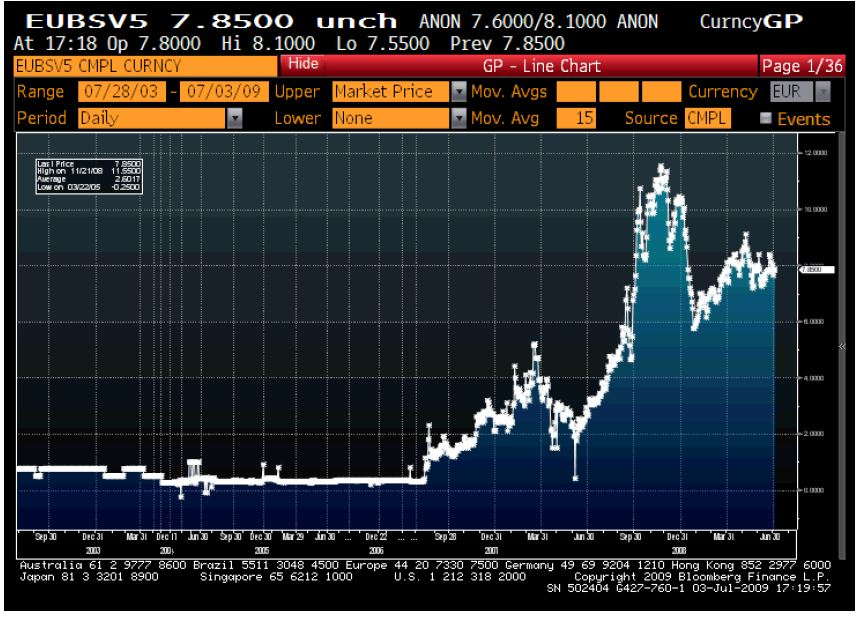
\includegraphics[scale=0.8]{tenor_premium}
\caption{Basis swap 3M vs 6M premium}
\label{fig:tenor_premium}
\end{figure}

a change of structure, but not correlation among different tenor appeared, which led to phenomenons like the difference between implied forward rate (forward rate from the in-house term structure) and market forward rate (quoted on the market) and therefore Forward Rate Agreement mispricing:

\begin{figure}[H]
\centering
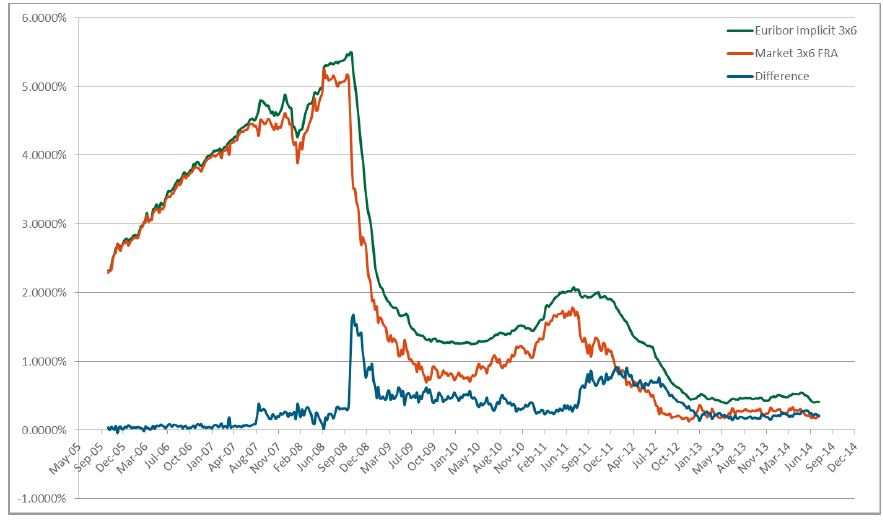
\includegraphics[scale=0.8]{implied_market_forward}
\caption{Implied FRA vs Market FRA}
\label{fig:implied_market_forward}
\end{figure}

Given these considerations, a framework for estimating these new curves was required. The chosen method is the bootstrapping, a numerical procedure that allows to retrieve a term structure such that the market quotes used in the process are exactly or with the minimum error repriced.
The bootstrap vademecum core principles requires:

\begin{itemize}
    \item smoothness as term structure quality indicator, the most granular representation of the curve is its instantaneous forward one, that in the real world corresponds to look at overnight forward rate applying \eqref{eq:no_arbitrage_forward_sc_int} with $t_{2} = t_{1} + 1 \text{day}$;
    
    \item homogeneous instruments: it means that in order to bootstrap an x tenor curve the algorithm has to be fed with the corresponding instruments in term of tenor in order to incorporate the correct maturity and credit premia;
    
    \item unique discounting curve: before the crisis discounting and forwarding curve coincided, after rising of multiple curves it was needed to chose a discounting curve. Initially each curve was discounted using itself (endogenous discounting), but clearly this was not reasonable. Indeed, given that 1\$ tomorrow is worth the same independently from what curve it is considered, it should be found a unique discounting curve.
    Given that the interest rate derivatives world is based on collateralization  and given that on collateral account is paid the ON rate, it makes sense that the cost of money and therefore the discounting curve should be retrieved on the overnight one (exogenous discounting);
    
    \item exclusion of deposit in bootstrap procedure: according to the previous considerations and given that deposits are not collateralized it makes no sense including them in the procedure. Instead, it is possible to include the so called ``synthetic deposits" in order to populate the part of curve with tenor smaller than the one of the bootstrapped curve;
    
    \item choice of bootstrap method: exact fit or best fit. While the former lead to an exact repricing of market quote, the second just try to achieve the best fit as possible. The main idea is that ``a term structure that cannot perfectly reprice the instruments which is looking at during the bootstrap it is fragile and seems not reliable for further uses", therefore an exact fit approach is preferred.
    \item choice of interpolation scheme. A global interpolator allows to preserve curve shape, while a local one exchanges a better shape with easiness of implementation and interpretation. The former, although bringing complexity, is preferred. 
\end{itemize}

Understood which are the best practices on the market, before proceeding toward the implementation, there are common problems that need to be addressed in order to perfectly get the idea of how a bootstrapping algorithm works:

\begin{itemize}

\item information short: if the aim is to bootstrap a curve with a tenor greater than ON, it means that in the first part of the curve up to the first market quote there will be a short of information, therefore the 
quant needs to understand how to manage it. Different solution have been implemented, among those it is spread the use of synthetic deposits, which roughly speaking mimic the shape of ON curve adding a basis in order to match the $x$ tenor modelled curve magnitude; 

\item liquidity necessity: given a liquidity need, that arises because of regulation constraints, in the end of year, or more generally each time that liquidity requirements come, a leap on the ON curve is observed. It is transmitted to a greater $x$ tenor modelled curve diminishing the smoothness. This matter required a particular estimation technique which can easily lead to an overall estimation error;

\item missing pillar: given $n$ market quotes which help to model their respective curve, how is it possible to deal with those curve pillar which are not reflected in them, but can be useful to evaluate particular instruments? The answer is: interpolating. This point opens new debating about possible practitioner's solutions. The first choice could be to use a local interpolation scheme, it means that the searched point is fully described by 2 points which lay next to it, for example the linear interpolation belongs to this family. Unfortunately this approach do not preserve the curve shape, therefore advanced interpolations scheme should be employed and they are called global, because the interpolated point depends on the global shape of the curve, dependencies exist among each point of the curve. Among them, the one which leads to optimal results is the monotonic cubic, but this algorithm may have problem of spurious convexity or lack of monotonicity, that can be erased applying a filter as the Hyman one.

\end{itemize}

\section{The algorithm}

Given the above explained background where the bootstrap algorithm takes roots, it is possible to proceed with the explanation relying on the QuantLib implementation.

The main elements that compete in bootstrapping procedure are:

\begin{enumerate}
    \item a vector of not overlapping market quotes (deposit, FRA, futures, Swap) $\textbf{Q} =\{q_{1},q_{2}\dots q_{n}\}$;
    \item trait \textbf{T}, it is the form of the rate used in the interpolation (discount factor, forward rate, instantaneous forward rate);
    \item interpolation type \textbf{I} (linear, cubic spline, ecc \dots);
    \item type of bootstrapping \textbf{B} (iterative bootstrap, local bootstrap);
    \item a guess of the curve points $\textbf{P} =\{p_{1},p_{2}\dots p_{n}\}$.
\end{enumerate}

In the following the iterative bootstrap (B is given) algorithm is sketched.

Firstly, the process is recursive and incremental: it means that starts from the first pillar and evolves pillar by pillar up to the last one, corresponding to the last market date, and if the exit condition is still unsatisfied it restarts recursively up to its satisfaction. \footnote{For instance the maximum difference between the curve quotes before and after the bootstrap cycle needs to be lower than the accuracy or the reaching of the maximum number of iterations.}
Given that each $q_{i}$ instrument refers to a precise date and the set of dates is ordered, the algorithm starts cycling from the first available date, i.d the first pillar, which corresponds to the first element of Q. 
The first time an instrument enters in the process, for its corresponding pillar, a guess is provided \footnote{In the recursive loop the guess becomes the value from the previous iteration} and subsequently passed as inputs to the solver which tries to minimize the error function of the $q_{i}$ quote and the $r_{i}$ quote, which is implied (instrument dependent) in the currently bootstrapped term structure. 
For instance, given a quoted $q_{i}$ that corresponds to market FRA rate, that is quoted in term of its contractual fixed rate, the corresponding implied quote $r_{i}$ in the term structure has to be the same of it. This means zeroing the error function as below reported:

\begin{equation*}
   f(q_{i},r_{i})=0
\end{equation*}

In order to achieve this result the solver changes the guess/ previous value, the algorithm puts the new value in curve (at the height of the considered pillar), the curve is interpolated with the specified type of interpolation I on the decided form of rate T, then $r_{i}$ is computed and an error retrieved through $f(q_{i},r_{i})$.
Once the pillar has been changed, the algorithm steps ahead to the next pillar and it re-proposes the same solution.
Note: in this process the evaluation of each instrument depends on the I that has been chosen, because for evaluating instruments with fixing dates outside the quoted grid an interpolation is required. In particular case of global type, changing the pillar means to change the bootstrapped term structure. Because of this continuous mutant behavior the algorithm should evaluate recursively each pillar more than once in order to satisfy the already mentioned condition. 

The above reported was the QuantLib idea of bootstrapping, anyway, instead of repricing the quotes, it is possible to work on the term structure that allows zeroing the instruments net present value. In this case, the rationale is that in order to buy and sell today a given instrument its net present value should be zero, otherwise cannot there be a deal counterpart.

Concluding, the multiple curve bootstrap is fundamental not only as a finance principle, but also in the continuation of this research, because it has been used in abcd framework for building the legacy curves \footnote{Legacy curve refers to the bootstrapped curve that in the following is substituted by the new framework} that are both one of the metric with respect to evaluate the goodness of the new curves scheme together with a necessary step in order to build them.

\begin{algorithm}
	\caption{Iterative Bootstrapping algorithm}
	\label{alg:bootstrapping}
	\begin{algorithmic}[1]
	\Procedure{Bootstrapping}{T,I,Q}
	    \State $P\gets Interpolator(T,I)$
	    \State $P.quotes \gets guessedCurve$
		\For {$i \gets 1, maxNumberIterations$}
		\For {$j \gets 1, N$}
	    \State $\min (p_{j}) f(j,Q,R,P)$
		\EndFor
		\If {exitCondition}
		\State \textbf{return} P 
		\EndIf
		\EndFor
	\EndProcedure
	\end{algorithmic}
\end{algorithm}

\begin{algorithm}
	\caption{min}{}
	\label{alg:min}
	\begin{algorithmic}[1]
	\Procedure{min}{j,Q,R,P}
	   \For {$i \gets 1, maxNumberIterations$}
	   \If {$i==1$}
	   \State $p_{j} \gets guess$
	   \EndIf
	   \State P.interpolate
	   \State $r_{j}\gets P.impliedQuote(j)$
	   \If {$f(q_{j},r_{j}) < \epsilon$}
	   \State \textbf{return} $p_{j}$
	   \EndIf
	   \State $p_{j} \gets solver.updateValue()$
	   \EndFor
	\EndProcedure
	\end{algorithmic}
\end{algorithm}